% this TeX file provides an awesome example of how TeX will make super 
% awesome tables, at the cost of your of what happens when you try to make a
% table that is very complicated.
\documentclass[11pt]{article}

% Use wide margins, but not quite so wide as fullpage.sty
\marginparwidth 0.5in 
\oddsidemargin 0.25in 
\evensidemargin 0.25in 
\marginparsep 0.25in
\topmargin 0.25in
\textwidth 6in
\textheight 8in
% That's about enough definitions

% language input
\usepackage[utf8]{inputenc}
% multirow allows you to combine rows in columns
\usepackage{multirow}
% tabularx allows manual tweaking of column width
\usepackage{tabularx}
% insert images
\usepackage{graphicx}
\usepackage{float}
\usepackage{booktabs}
\graphicspath{ {images/} }

\begin{document}
% this is an alternate method of creating a title
%\hfill\vbox{\hbox{Gius, Mark}
%       \hbox{Cpe 456, Section 01}  
%       \hbox{Lab 1}    
%       \hbox{\today}}\par
%
%\bigskip
%\bigskip
\author{Vandré Leal Cândido}
\title{Wireshark Lab: TCP v6.0}
\maketitle

% 2. A first look at the captured trace
\section{A first look at the captured trace}

\par Answer the following questions, by opening the Wireshark captured packet file tcpethereal-trace-1 in
http://gaia.cs.umass.edu/wireshark-labs/wireshark-traces.zip (that is download the trace and open that
trace in Wireshark; see footnote 2). Whenever possible, when answering a question you should hand
 in a printout of the packet(s) within the trace that you used to answer the question asked. Annotate the 3
printout to explain your answer. To print a packet, use File - Print, choose Selected packet only, choose Packet summary line, and select the minimum amount of packet detail that you need to answer the question.

\begin{itemize}
	\setlength\itemsep{.5cm}

	\item
		\textit{What is the IP address and TCP port number used by the client computer (source) that is transferring the file to gaia.cs.umass.edu? To answer this question, it’s probably easiest to select an HTTP message and explore the details of the TCP packet used to carry this HTTP message, using the “details of the selected packet header window” (refer to Figure 2 in the “Getting Started with Wireshark” Lab if you’re uncertain about the Wireshark windows.}
		\par The IP address used by the client computer is 192.168.1.102 and the source TCP port number is 1161.
	
	\item
		\textit{What is the IP address of gaia.cs.umass.edu? On what port number is it sending and receiving TCP segments for this connection?}
		\par The IP address of gaia.cs.umass.edu is 128.119.245.12 and the TCP port is 80.
		
		\begin{figure}[H]
		\centering
		\caption{tcpethereal-trace-1}
		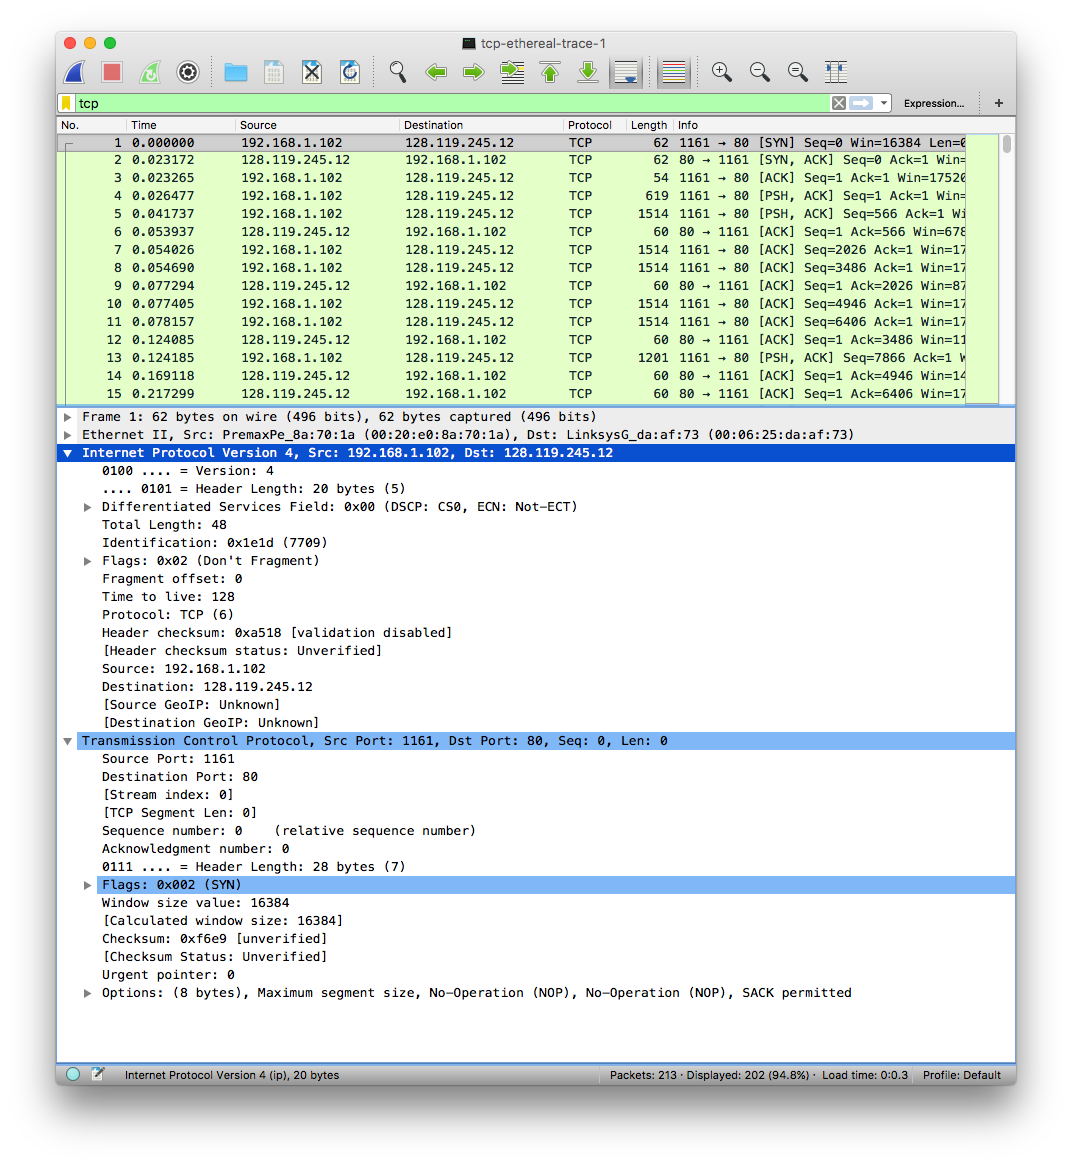
\includegraphics[width=400px]{01}
		\end{figure}
	
\par If you have been able to create your own trace, answer the following question:

	\item
		\textit{What is the IP address and TCP port number used by your client computer (source) to transfer the file to gaia.cs.umass.edu?}
		\par The IP address used by my computer is 192.168.0.15 and the TCP port is 64813.
		
		\begin{figure}[H]
		\centering
		\caption{tcplocal-trace-1}
		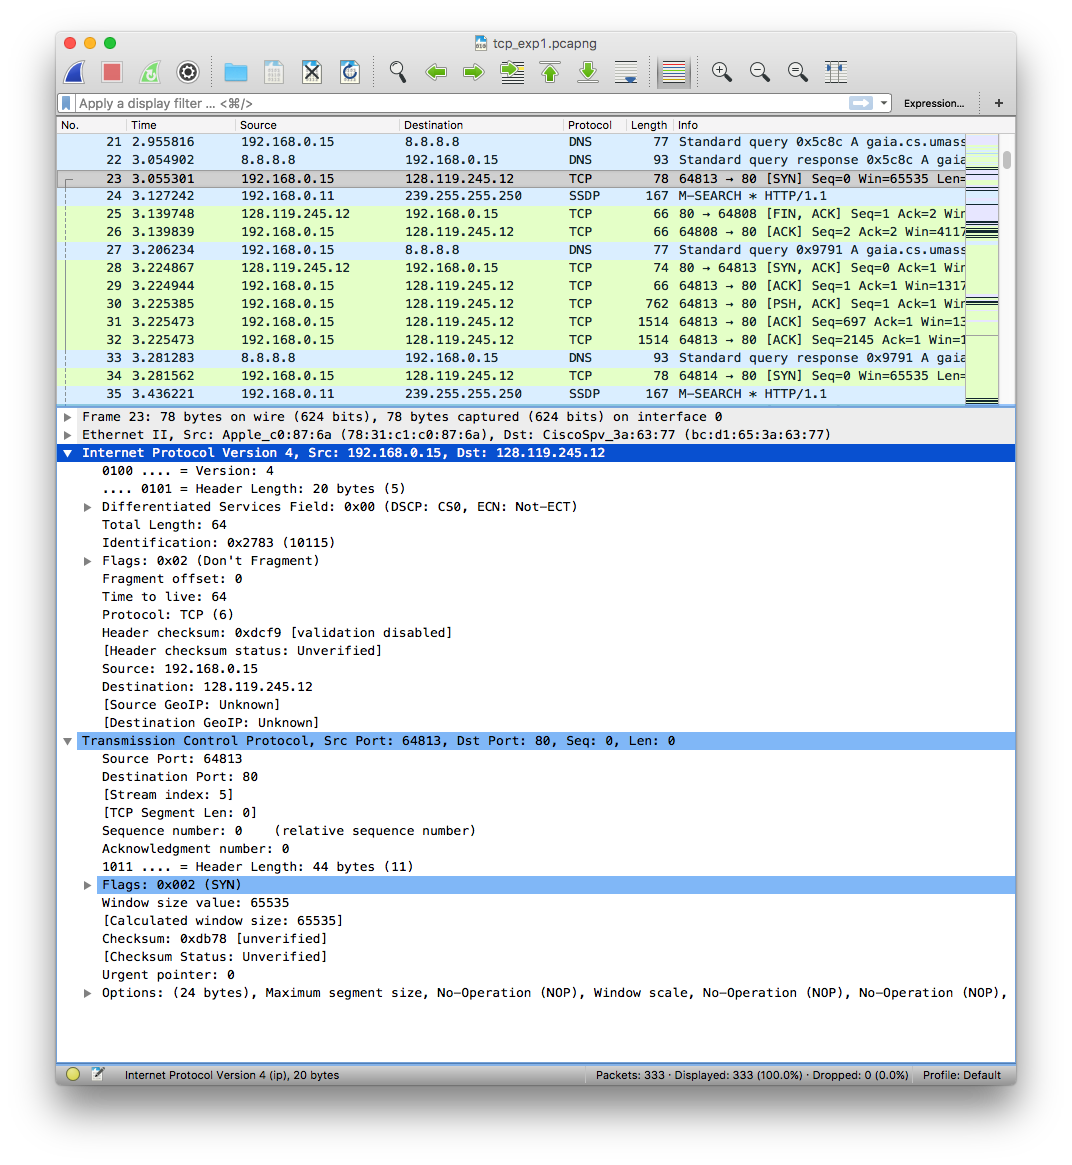
\includegraphics[width=400px]{02}
		\end{figure}
	
\end{itemize}

\pagebreak

% 3. TCP Basics
\section{TCP Basics}

\begin{itemize}
	\setlength\itemsep{.5cm}

	\item
		\textit{What is the sequence number of the TCP SYN segment that is used to initiate the TCP connection between the client computer and gaia.cs.umass.edu? What is it in the segment that identifies the segment as a SYN segment?}
		\par The sequence number used to initiate the TCP connection is 0. The \textbf{SYN} flag highlighted below indicates that the segment is a SYN segment.
		
		\begin{figure}[H]
		\centering
		\caption{tcplocal-trace-1 (Question 04)}
		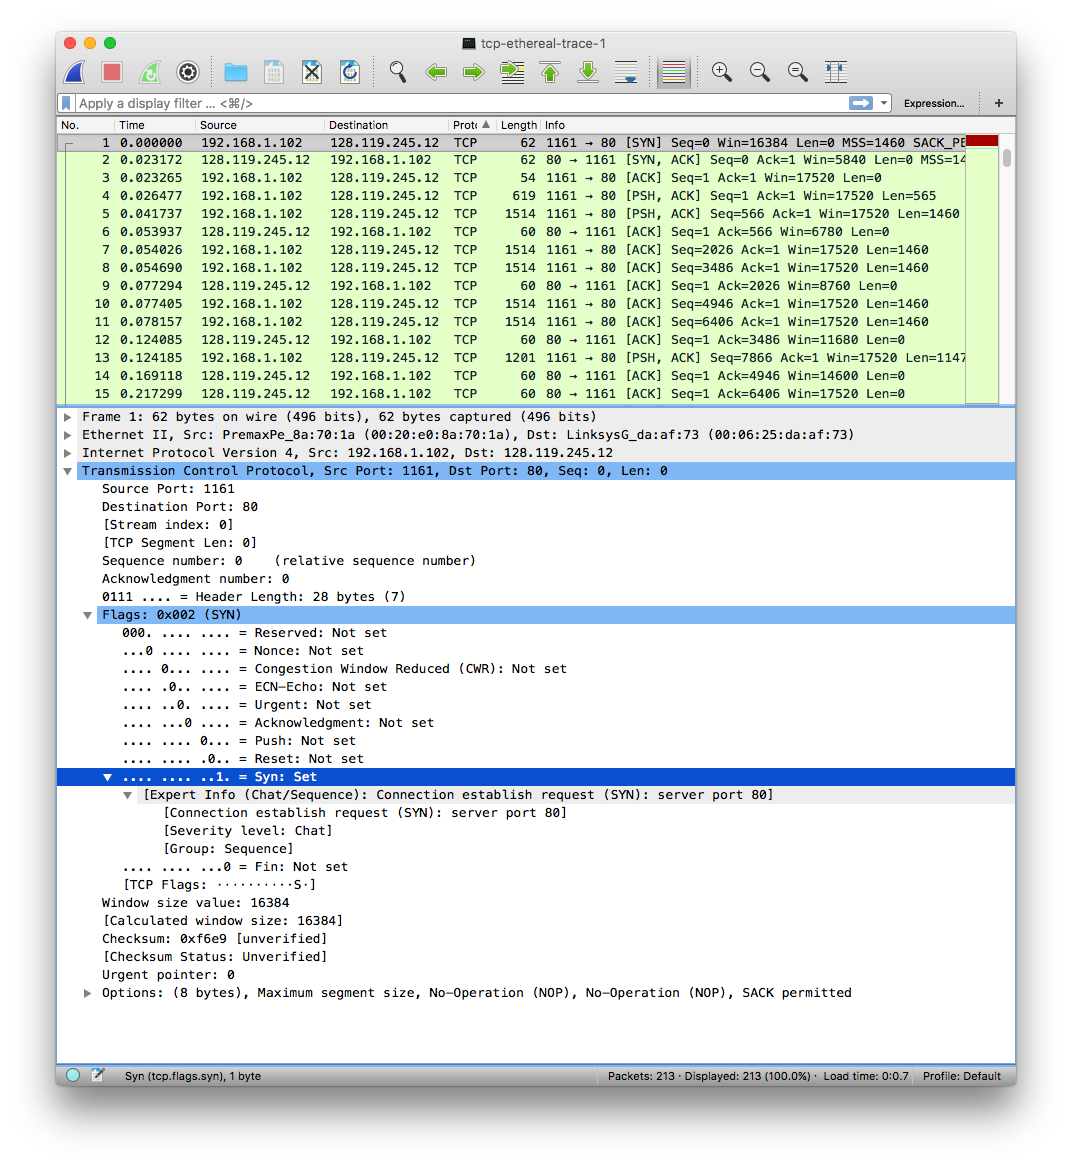
\includegraphics[width=400px]{03}
		\end{figure}

	\item
		\textit{What is the sequence number of the SYNACK segment sent by gaia.cs.umass.edu to the client computer in reply to the SYN? What is the value of the Acknowledgement field in the SYNACK segment? How did gaia.cs.umass.edu determine that value? What is it in the segment that identifies the segment as a SYNACK segment?}
		\par The sequence number of the SYNACK segment sent by gaia.cs.umass.edu to the client computer is 0. The value of the ACK filed in the SYNACK segment is 1 as highlighted below. gaia.cs.umass.edu determined the value by adding 1 to the initial sequence number of SYN segment (0). Both the \textbf{SYN} and the \textbf{Acknoledgment} flags are set to 1, which indicates that this is a SYNACK segment.
		
		\begin{figure}[H]
		\centering
		\caption{tcplocal-trace-1 (Question 05)}
		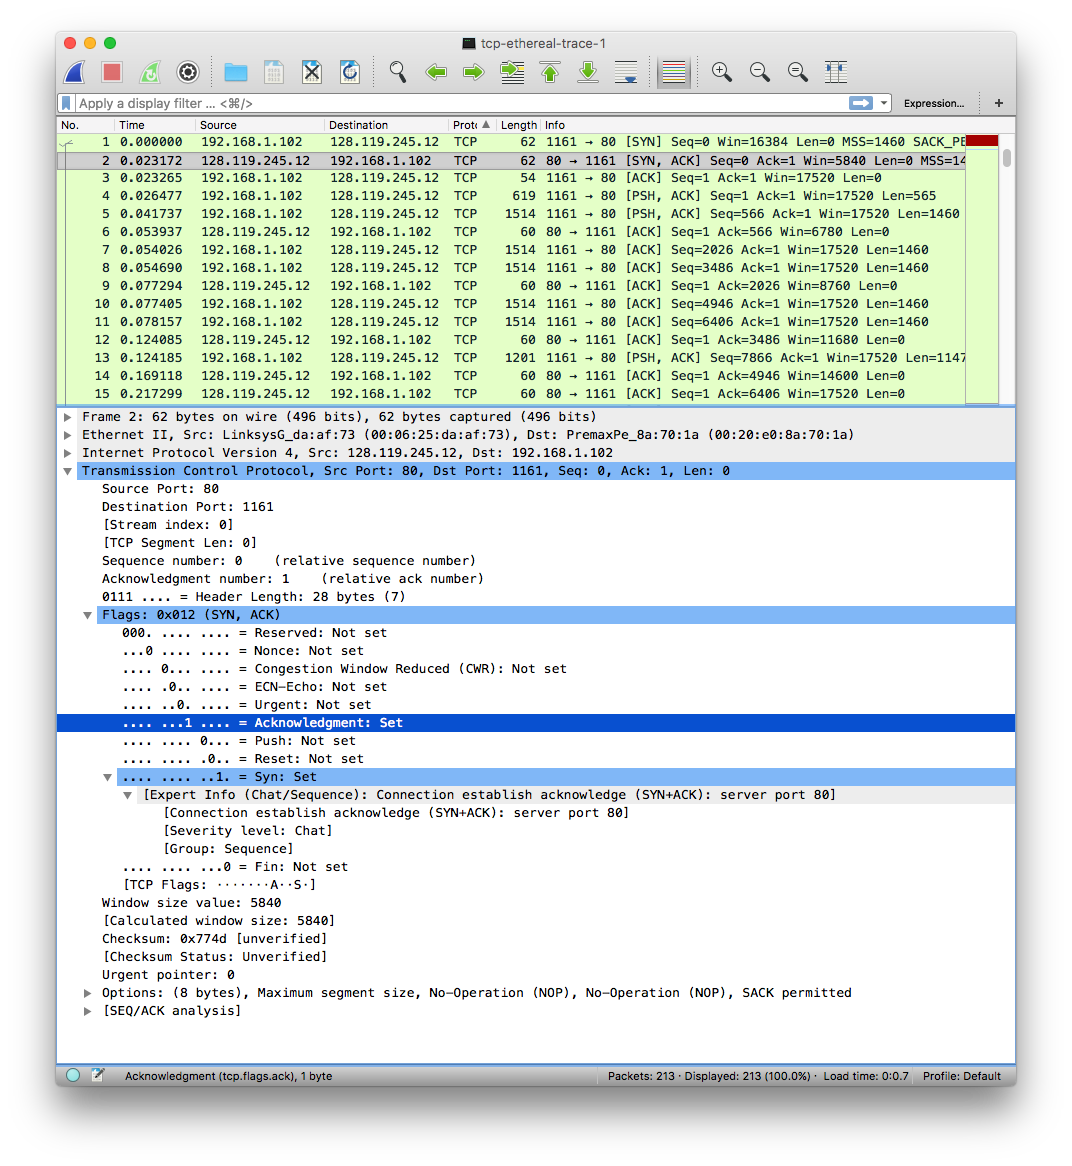
\includegraphics[width=380px]{04}
		\end{figure}
		
	\item
		\textit{What is the sequence number of the TCP segment containing the HTTP POST command? Note that in order to find the POST command, you’ll need to dig into the packet content field at the bottom of the Wireshark window, looking for a segment with a “POST” within its DATA field.}
		\par The sequence number of the TCP segment containing the POST command is 1. The segment is highlighted below and has the flag \textbf{Push} set to 1 indicating that the client is sending data.
		
		\begin{figure}[H]
		\centering
		\caption{tcplocal-trace-1 (Question 06)}
		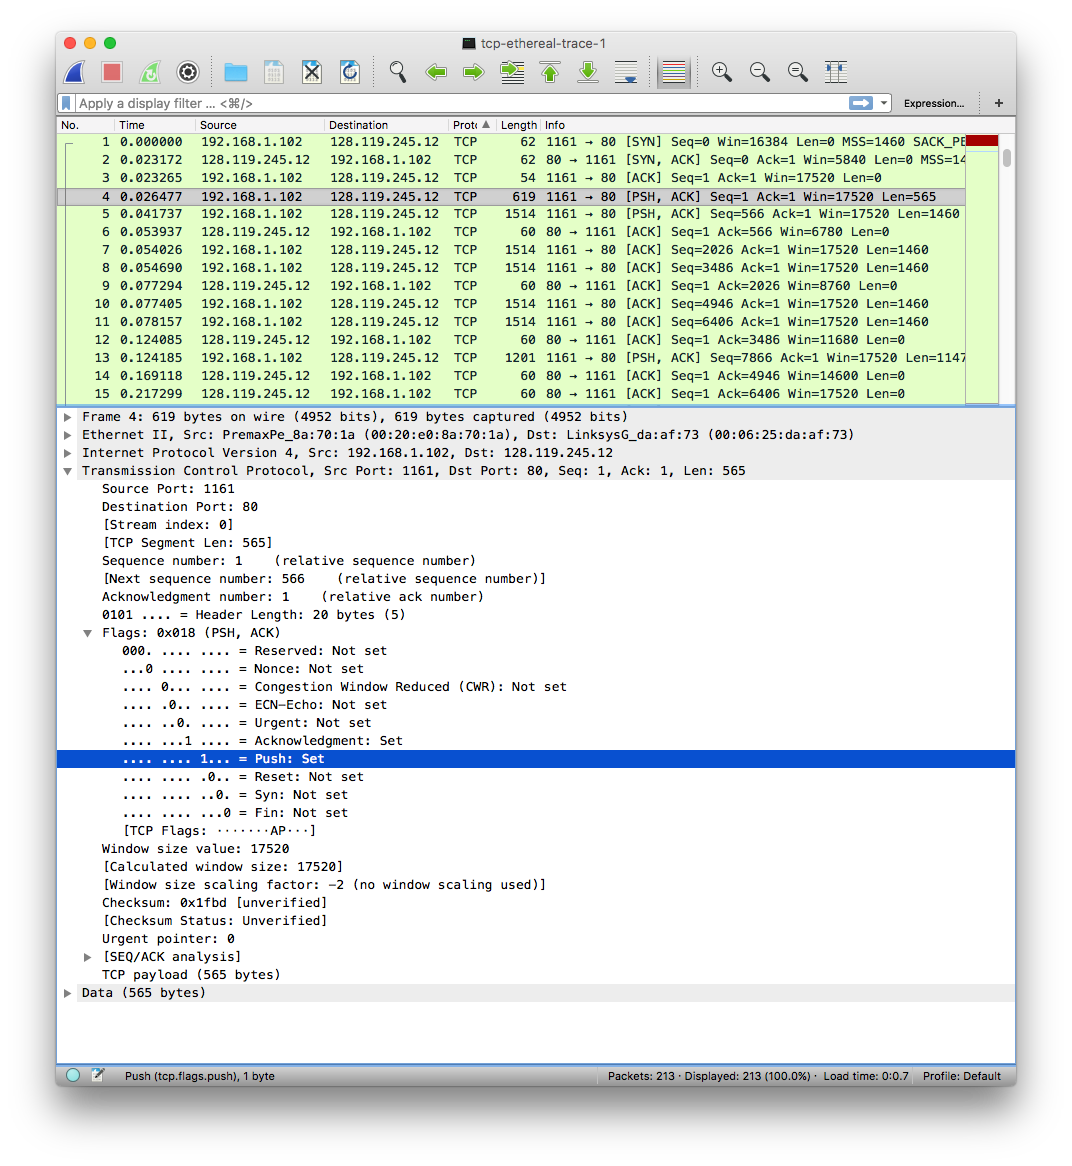
\includegraphics[width=400px]{05}
		\end{figure}
		
	\item
		\textit{Consider the TCP segment containing the HTTP POST as the first segment in the TCP connection. What are the sequence numbers of the first six segments in the TCP connection (including the segment containing the HTTP POST)? At what time was each segment sent? When was the ACK for each segment received? Given the difference between when each TCP segment was sent, and when its acknowledgement was received, what is the RTT value for each of the six segments? What is the EstimatedRTT value (see Section 3.5.3, page 239 in text) after the receipt of each ACK? Assume that the value of the EstimatedRTT is equal to the measured RTT for the first segment, and then is computed using the EstimatedRTT equation on page 239 for all subsequent segments.}
		\par The sequence numbers of the first six segments in the TCP connection are 1, 566, 2026, 3486, 4946 and 6406 (frames 4, 5, 7, 8, 9 and 10) in the trace. The ACK received for each one the segments are frames 6, 9, 12, 14, 15 and 16, respectively.

\begin{table}[H]
\centering
\caption{RTT values (seconds)}
\label{rtt-values}
\begin{tabular}{@{}lllll@{}}
\toprule
Segment & Frame & Sent time (seconds) & ACK received (seconds) & RTT (seconds) \\ \midrule
1       & 4     & 0.026477            & 0.053937               & 0.02746       \\
2       & 5     & 0.041737            & 0.077294               & 0.035557      \\
3       & 7     & 0.054026            & 0.124085               & 0.070059      \\
4       & 8     & 0.054690            & 0.169118               & 0.11443       \\
5       & 10    & 0.077405            & 0.217299               & 0.13989       \\
6       & 11    & 0.078157            & 0.267802               & 0.18964       \\ \bottomrule
\end{tabular}
\end{table}

\par The EstimatedRTT equation on page 239 is
\par \textit{EstimatedRTT = 0.875 * EstimatedRTT + 0.125 * SampleRTT}
\newline

\par Segment 1: \textit{EstimatedRTT = 0.02746 secs}
\newline

\par Segment 2: \textit{EstimatedRTT = 0.875 * 0.02746 + 0.125 * 0.035557 = 0.0285 secs}
\newline

\par Segment 3: \textit{EstimatedRTT = 0.875 * 0.0285 + 0.125 * 0.070059 = 0.0337 secs}
\newline

\par Segment 4: \textit{EstimatedRTT = 0.875 * 0.0337+ 0.125 * 0.11443 = 0.0438 secs}
\newline

\par Segment 5: \textit{EstimatedRTT = 0.875 * 0.0438 + 0.125 * 0.13989 = 0.0558 secs}
\newline

\par Segment 6: \textit{EstimatedRTT = 0.875 * 0.0558 + 0.125 * 0.18964 = 0.0725 secs}
\newline

		\begin{figure}[H]
		\centering
		\caption{tcplocal-trace-1 (Question 07)}
		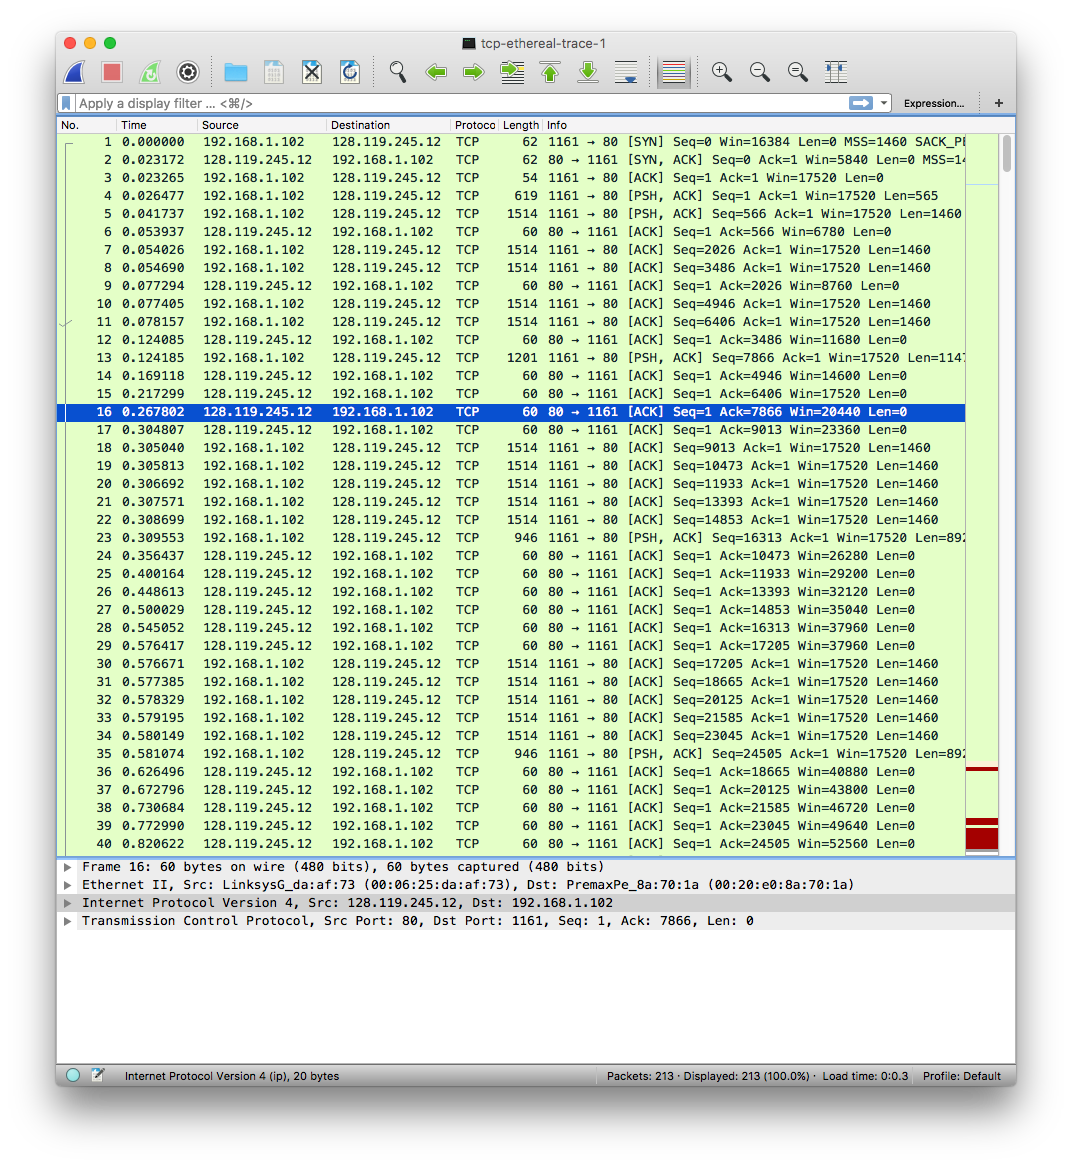
\includegraphics[width=\textwidth]{06}
		\end{figure}
		
\pagebreak

	\item
		\textit{What is the length of each of the first six TCP segments?}
		\par The length of the first TCP segment (including the HTTP POST) is 565 bytes. The length of each one of the other five segments is 1460 bytes.  This value is included within the TCP section as highlighted below but can also be quickly identified by checking the value of \textbf{Len} in the column \textbf{Info} for each one of the segments in the trace. 
		
		\begin{figure}[H]
		\centering
		\caption{tcplocal-trace-1 (Question 08)}
		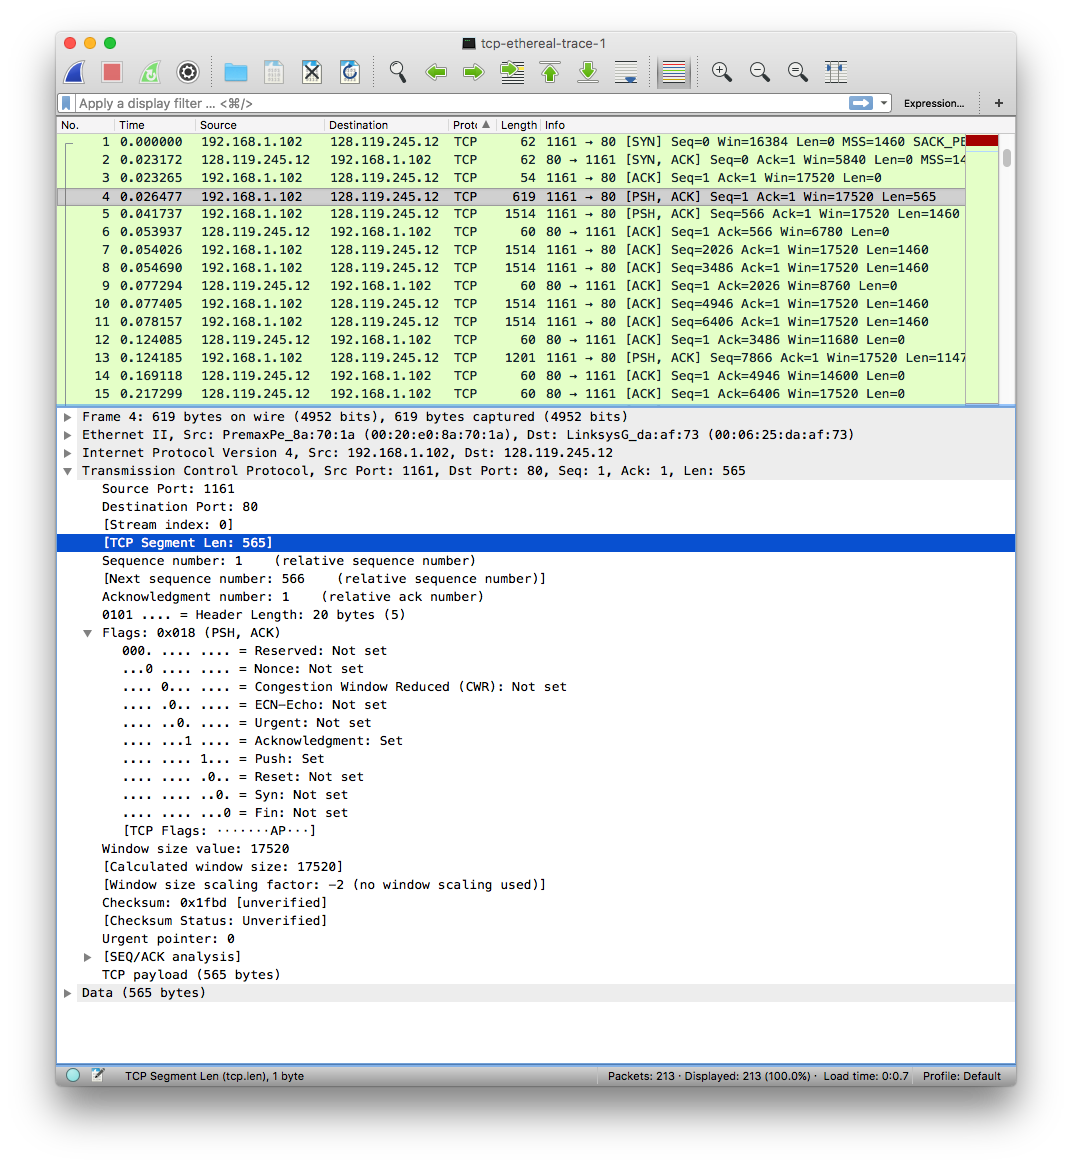
\includegraphics[width=400px]{07}
		\end{figure}
		
	\item
		\textit{What is the minimum amount of available buffer space advertised at the received for the
entire trace? Does the lack of receiver buffer space ever throttle the sender?}
		\par The minimum amount of buffer space advertised at the received (gaia.cs.umass.edu) for the entire trace is 5840 bytes as indicated by the field \textbf{Window size value} in the first ACK. The window size value grows until it reaches the value 62780 bytes as indicated in the last POST segment. By inspecting the trace it doesn't seem like the sender ever throttle due to lack of buffer space.
		
		\begin{figure}[H]
		\centering
		\caption{tcplocal-trace-1 (Question 09 - First ACK)}
		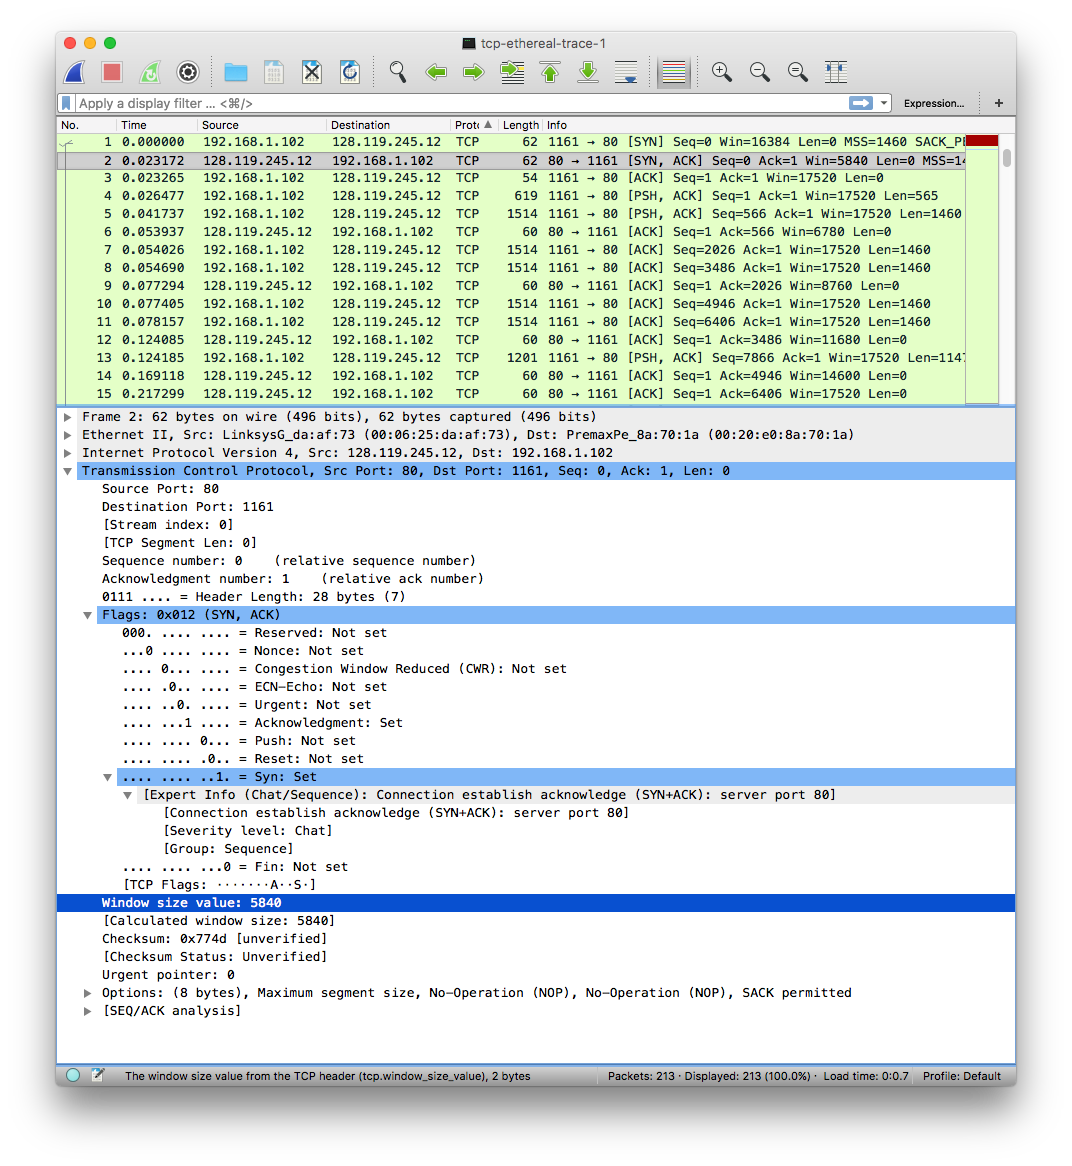
\includegraphics[width=400px]{08}
		\end{figure}
		
		\begin{figure}[H]
		\centering
		\caption{tcplocal-trace-1 (Question 09 - Last POST segment)}
		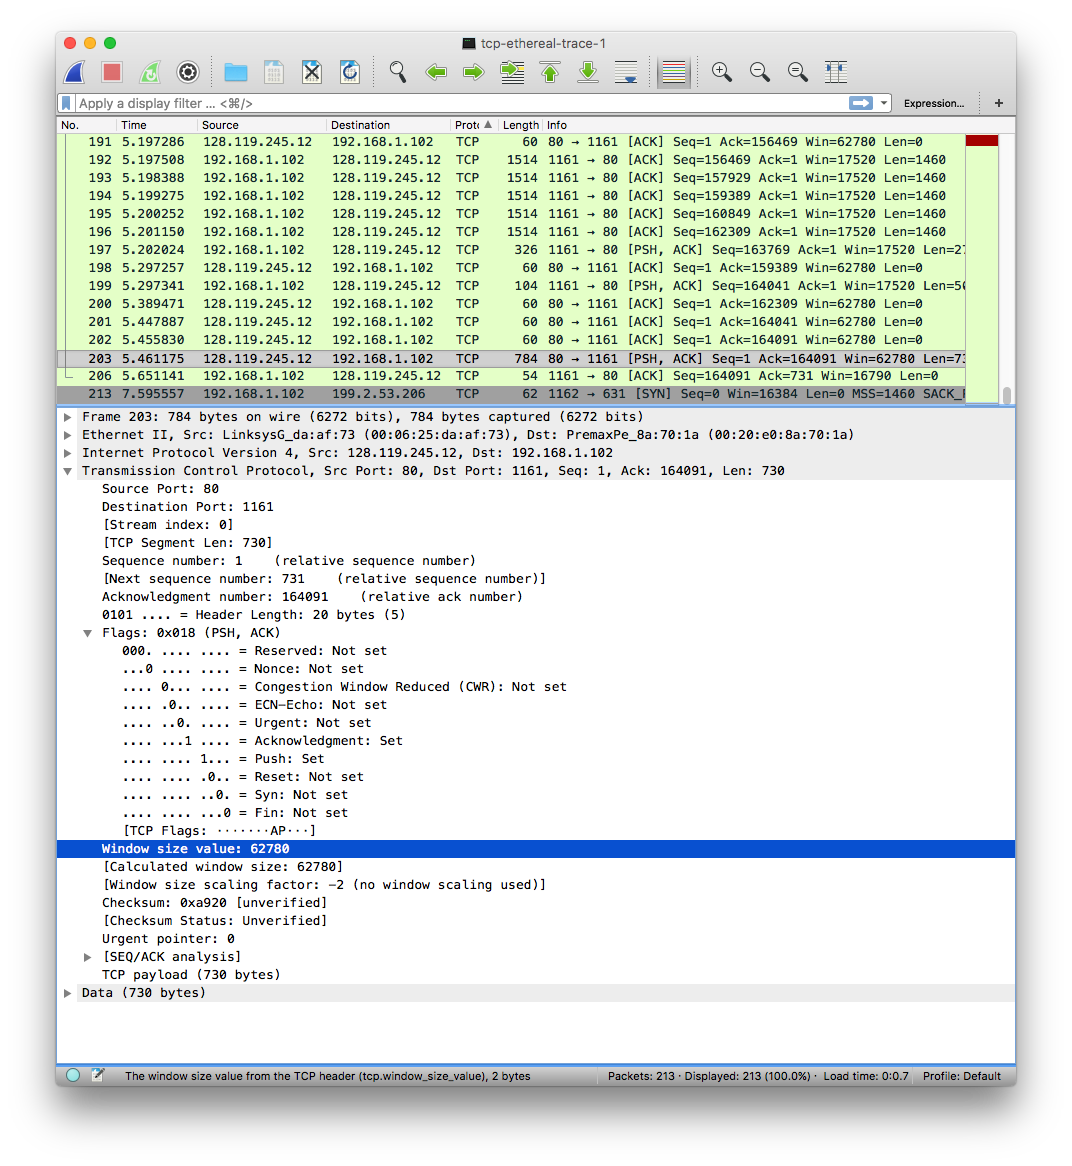
\includegraphics[width=400px]{09}
		\end{figure}

	\item
		\textit{Are there any retransmitted segments in the trace file? What did you check for (in the trace)
in order to answer this question?}
		\par There are no retransmitted segments in the trace file. There aren't any wireshark frames highlighted as retransmitted [TCP Retransmission]. Additionally, all sequence numbers increases as packets are sent. When a segment is retransmitted, the sequence number of the segment is smaller than the sequence number of its nearby segments.
		
	\item
		\textit{How much data does the receiver typically acknowledge in an ACK? Can you identify cases
where the receiver is ACKing every other received segment (see Table 3.2 on page 247 in the
text).}
		\par The receiver typically acknowledge 1460 bytes in an ACK.
		
	\item
		\textit{What is the throughput (bytes transferred per unit time) for the TCP connection? Explain how
you calculated this value.}
		\par The average throughput is computed as the ratio between the total amount data and the total transmission time.
		\newline
		
		\par \textbf{Total amount data:}
		\newline Sequence number of the last ACK minus the seq number of the first TCP segment
		\newline 164091 - 1
		\newline 164090 bytes.
		\newline
		
		\par \textbf{Total transmission time:}
		\newline Time instant of the last ACK minus the time instant of the first TCP segment
		\newline 5.455830 - 0.026477
		\newline 5.4294 seconds.
		\newline
		
		\par Therefore, the throughput for the TCP connection is 164090/5.4294 = \textbf{30.222 Kbs/sec}.

\end{itemize}

\pagebreak

% 4. TCP congestion control in action
\section{TCP congestion control in action}

\begin{itemize}
	\setlength\itemsep{.5cm}

	\item
		\textit{Use the Time-Sequence-Graph(Stevens) plotting tool to view the sequence number versus time plot of segments being sent from the client to the gaia.cs.umass.edu server. Can you identify where TCP’s slowstart phase begins and ends, and where congestion avoidance takes over? Comment on ways in which the measured data differs from the idealized behavior of TCP that we’ve studied in the text.}
		
		\begin{figure}[H]
		\centering
		\caption{tcplocal-trace-1 (Question 13 - Time-Sequence-Graph(Stevens))}
		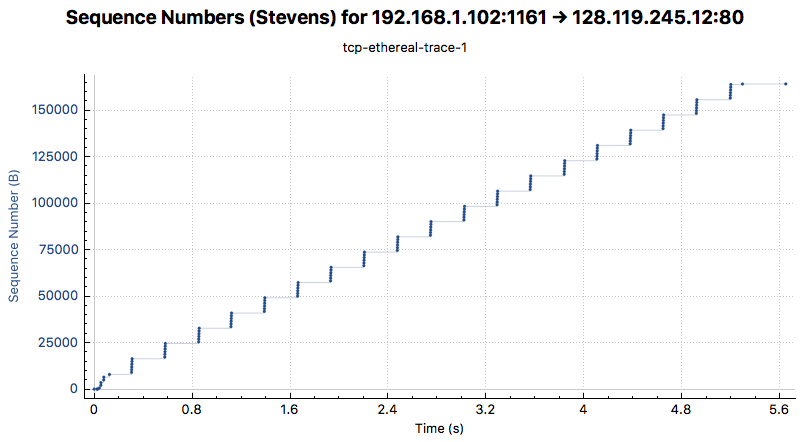
\includegraphics[width=\textwidth]{10}
		\end{figure}

	\item
		\textit{Answer each of two questions above for the trace that you have gathered when you transferred a file from your computer to gaia.cs.umass.edu}
		\par There's no way to determine the end of the slow start phase and the start of the congestion avoidance since the client is not sending enough data to force a congestion state. The client stops transmitting data before any congestion.

\end{itemize}

\end{document}
